\documentclass[a4paper,enabledeprecatedfontcommands]{scrartcl}
\usepackage[ngerman]{babel}
\usepackage[T1]{fontenc}
\usepackage[utf8]{inputenc}
\usepackage{graphicx}
\usepackage{color}
\usepackage{colortbl}
\usepackage{xcolor}
\usepackage{helvet}
\renewcommand{\familydefault}{\sfdefault}
\usepackage{amsmath,amssymb,amsthm,textcomp}
\usepackage{tikz}
\usepackage[a4paper,head=1.5cm,bottom=2.5cm,left=25mm,right=25mm]{geometry}

\setlength\parindent{0pt}
\newcommand{\titleline}{\rule{\linewidth}{0.5pt}}

\makeatletter
\renewcommand{\maketitle}{
\begin{center}
\vspace{2ex}
{\huge \textsc{\@title}}
\vspace{1ex}
\\
\titleline\\
\@author \hfill \@date
\vspace{3ex}
\end{center}
}
\makeatother
\usepackage{fancyhdr}
\pagestyle{fancy}
\lhead{}
\chead{}
\rhead{}
\lfoot{}
\cfoot{}
\rfoot{Seite \thepage}
\renewcommand{\headrulewidth}{0pt}
\renewcommand{\footrulewidth}{0pt}
\usepackage{listings}

\definecolor{Titelfarbe}{HTML}{CF4A30}
\definecolor{Titelhintergrundfarbe}{RGB}{171, 37, 36}
\definecolor{ivory}{RGB}{255,255,240}
\definecolor{Purple}{HTML}{911146}
\definecolor{Orange}{HTML}{CF4A30}
\definecolor{LightOrange}{HTML}{FFCF9E}
\definecolor{quoteColor}{RGB}{255,255,240}
\definecolor{keywordColor}{HTML}{0033B3}

\lstset{
	keywordstyle=\ttfamily\color{keywordColor}\bfseries, 
	backgroundcolor=\color{ivory},
	commentstyle=\ttfamily\color{red}, 
	stringstyle=\ttfamily,
	numberstyle=\normalsize, 
	basicstyle=\normalsize\ttfamily, 
	showstringspaces=false, 
	breaklines=true, 
	language=Java
}


\title{Übungen: Black-Box-Testverfahren}
\author{Markus Flingelli}
\date{\today}

\begin{document}
\maketitle

\section*{Aufgabe 1}
Ein Programm Mengenbeziehungstest muss geprüft werden. Diesem Programm werden zwei Mengen $A$ und $B$ übergeben. Die folgende Tabelle spezifiziert dabei, unter welchen Bedigungen, welche Ausgabe verfolgen soll:

\vspace{.3cm}

\begin{tabular}{|l|l|}
\hline
\textbf{Bedingung} & \textbf{Ausgabe}\\ \hline
$A \cup B = A \cap B$ & Gleichheit\\ \hline
$A \subset B \lor B \subset B$ & Echte Teilmenge\\ \hline
$A \cap B \neq \emptyset$ & Überdeckung\\ \hline
$A \cap B = \emptyset$ & Disjunktion\\ \hline
\end{tabular}

\subsection*{Aufgabe 1.1}
Ist die Spezifikation ausreichend? Begründe Deine Aussage.

\subsection*{Aufgabe 1.2}
Wie viele Testfälle ergeben sich aus der Spezifikation. Begründe Deine Aussage.

\newpage
\section*{Aufgabe 2}

Folgende Anforderung gilt für eine Webanwendung: Die Anzeige der Web-Anwendung soll auf Geräten mit folgenden Auflösungen eines Displays erfolgen können:

\begin{itemize}
  \item 640 x 480
  \item 1280 x 1024
  \item 1600 x 900
  \item 2048 x 1536
  \item 5120 x 2880
\end{itemize}

Wie viele gültige Äquivalenzklassen gibt es? Begründe Deine Aussage.

\newpage
\section*{Aufgabe 3}
Innerorts gilt folgender Bußgeldkatalog (Stand 27.05.2020). Die Angabe der Geschwindigkeit erfolgt ganzzahlig:

\vspace{.3cm}

\begin{tabular}{|l|r|}
\hline
\textbf{Geschwindigkeitsüberschreitung} & \textbf{Bußgeld} \\ \hline\hline
1 - 10 km/h                      & 15 €    \\ \hline
11 – 15 km/h 	                 & 25 €	   \\ \hline
16 – 20 km/h 	                 & 35 €	   \\ \hline
21 – 25 km/h 	                 & 80 €	   \\ \hline
26 – 30 km/h 	                 & 100 €   \\ \hline
31 – 40 km/h 	                 & 160 €   \\ \hline
41 – 50 km/h 	                 & 200 €   \\ \hline
51 – 60 km/h 	                 & 280 €   \\ \hline
61 – 70 km/h 	                 & 480 €   \\ \hline
Über 70 km/h 	                 & 680 €   \\ \hline
\end{tabular}

\subsection*{Aufgabe 3.1}
Bestimme alle Äquivalenzklassen auf Basis der Spezifikation.

\subsection*{Aufgabe 3.2}
Erstelle eine neue Testklasse mit Testmethoden, welche für je einen Vertreter der Äquivalenzen einen Test implementiert.

In dieser Übung soll das Verfahren \textit{Test Driven Development} verwendet werden, d.h zunächst sollen die Tests implementiert werden und anschließend erst die Methode.

\subsection*{Aufgabe 3.3}
Erstelle eine neue Testklasse mit den notwendigen Testmethoden auf Basis der Grenzwertanalyse.

\newpage
\section*{Aufgabe 4}
Ein Gastwirt hat Probleme mit der Zahlungsmoral einer Gäste. Einer seiner Gäste, ein Informatiker, schlägt ihm vor, folgendermaßen vorzugehen:

\begin{enumerate}
\item Wenn ein Kunde jünger als 18 Jahre alt ist und nicht bezahlen kann, rufe dessen Eltern an.
\item Wenn ein Kunde 18 Jahre und älter ist, kein Stammkunde ist und nicht bezahlen kann, dann rufe die Polizei an.
\item Wenn der Kunde 18 Jahre und älter ist und Stammkunde ist und den Rechnungsbetrag nicht bezahlen kann, kann er diesen aufschreiben lassen.
\end{enumerate}

\begin{tabular}{|l|l|l|l|l|l|l|l|l|l|}
\hline
 & & R1 & R2 & R3 & R4 & R5 & R6 & R7 & R8\\\hline \hline
B1 & Kunde jünger als 18 Jahre?  & J & J & J & J & N & N & N & N \\ \hline
B2 & Kunde kann Betrag bezahlen? & J & J & N & N & J & J & N & N \\ \hline 
B3 & Kunde ist Stammkunde        & J & N & J & N & J & N & J & N \\ \hline \hline
A1 & Bezahlen der Rechnung       &   &   &   &   &   &   &   &   \\ \hline 
A2 & Anruf bei den Eltern        &   &   &   &   &   &   &   &   \\ \hline
A3 & Anruf bei der Polizei       &   &   &   &   &   &   &   &   \\ \hline
A4 & Aufschreiben des Betrags    &   &   &   &   &   &   &   &   \\ \hline
\end{tabular}

\subsection*{Aufgabe 4.1}
Trage in die Entscheidungstabelle für jede mögliche Entscheidung die erwartete Aktion ein.

\subsection*{Aufgabe 4.2}
Gibt es Testfälle, die sich zusammenfassen lassen und wenn ja, welche sind das? Wie viele Testfälle ergeben sich mindestens?

\newpage
\section*{Aufgabe 5}

Gegeben ist folgendes Zustandsübergangsdiagramm:

\begin{center}
\begin{figure}[ht]
  \centering
  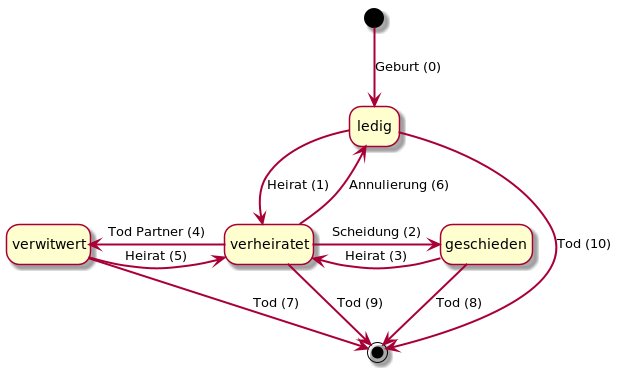
\includegraphics[width=\textwidth]{beziehungen.png}
\end{figure}
\end{center}

Bestimme die Anzahl an Testfällen, die mindestens notwendig ist, um alle Zustandsübergänge mindestens einmal getestet zu haben!

\end{document}